% chktex-file 8
\section{Exercise 2}

\subsection*{Part (a)}

\begin{figure}[H]
    \centering
    \def\edgebending{0cm}
\def\loopsize{0.5cm}
\definecolor{edgecolor}{RGB}{57, 0, 19}
\tikzstyle{matrix of math nodes}=[%
    matrix of nodes,
    nodes={%
     execute at begin node=$,%
     execute at end node=$%
    }%
  ]
\begin{tikzpicture}[scale=0.7,
    vertex/.style={fill = purple, circle, text = white, font=\bfseries},
    arc/.style={draw,ultra thick,->, shorten >=0.05cm, bend right = \edgebending, edgecolor},
    loop/.style={->, shorten > = 0.1cm, ultra thick, edgecolor}
    ]

    \newcommand{\coords}{
        (7, -3),
        (-7, -3),
        (0, 5),
        (0, 2),
        (-3, -2),
        (3, -2)
    }

    \newcommand{\adjmatrix}{
        {0.0, 1.0, 0.0, 1.0, 0.0, 0.0},
        {0.0, 0.0, 1.0, 0.0, 0.0, 0.0},
        {1.0, 0.0, 0.0, 0.0, 0.0, 0.0},
        {0.0, 1.0, 1.0, 0.0, 1.0, 0.0},
        {0.0, 0.0, 0.0, 0.0, 0.0, 1.0},
        {0.0, 0.0, 0.0, 1.0, 0.0, 0.0},
    }

    \newcommand{\labelmatrix}{
        {0.0, 1/2, 0.0, 1/2, 0.0, 0.0},
        {0.0, 0.0, 1  , 0.0, 0.0, 0.0},
        {1  , 0.0, 0.0, 0.0, 0.0, 0.0},
        {0.0, 1/3, 1/3, 0.0, 1/3, 0.0},
        {0.0, 0.0, 0.0, 0.0, 0.0, 1  },
        {0.0, 0.0, 0.0, 1  , 0.0, 0.0},
    }

    \newcommand{\getmatrixitem}[2]{%
    \StrBetween[#2,#1]{\labelmatrix}{, }{, }%
}


    % Define vertices
    \foreach [count = \i] \pos in \coords {
        \pgfmathsetmacro{\nodeangle}{round(90-atan2(\pos))}
        \ifnum\i=1
            \xdef\anglelist{\nodeangle}
        \else
            \xdef\anglelist{\anglelist,\nodeangle}
        \fi
        \coordinate[at=\pos, name=p\i];
        \pgfmathsetmacro{\nodename}{int(\i-1)}
        \node[vertex, at=\pos, name=V\i]{\nodename};
    }
        
    % Define edges
    \foreach [count = \i] \row in \labelmatrix{
    \foreach [count = \j] \edgelabel in \row{
        \pgfmathsetmacro{\weight}{{\adjmatrix}[\i-1][\j-1]}
        % Weight > 0
        \pgfmathsetmacro{\edgeexists}{\weight != 0 ? 1 : 0}
        \ifnum\edgeexists>0
            \pgfmathsetmacro{\isloop}{\i-\j == 0 ? 1 : 0}
            \ifnum\isloop>0
                \pgfmathsetmacro{\nodeangle}{{\anglelist}[\i-1]}
                \pgfmathsetmacro{\outangle}{int(\nodeangle - 50)}
                \pgfmathsetmacro{\inangle}{int(\nodeangle + 50)}
                \draw[loop] (V\i) to [in=\outangle,out=\inangle,looseness=\loopsize] node[fill=white] {$\edgelabel$} (V\i);
            \else
                \draw[arc] (V\i) to node[fill=white, inner sep=1pt] {$\edgelabel$} (V\j);
            \fi            
        \fi
    }
    }
\end{tikzpicture}
\end{figure}

\[ \Pi = \left[ \begin{array}{ccccc}
    \alpha & 1-\alpha & 0 & 0 & 0\\
    0 & \beta & 1-\beta-\varepsilon & 0 & \varepsilon\\
    1-\gamma-\delta & 0 & \gamma & \delta & 0\\
    0 & 0 & 0 & 1 & 0\\
    0 & 0 & 0 & 0 & 1\\
\end{array} \right] \]


\subsection*{Part (b)}

It can be the case that $A,B,C \in M$ if $\alpha,\beta,\gamma = 1$ respectively. Otherwise, $M = \{D,E\}$. However, in every case the maximum state should always be $E$.

\subsection*{Part (c)}

I don't understand if the problem ask for the minimum state in all these five cases:
\begin{multicols}{2}
    \begin{enumerate}
        \item $m = A$
        \item $m = B$
        \item $m = C$
        \item $m = D$
    \end{enumerate}
\end{multicols}

Or if there's a typo and it's asking for the maximum, which should always be: 5. $m = E$. On every case we should encounter the same linear system, given by:

\[ \left\{\begin{array}{ccl}
    \sum_{k = 0}^{N^2} \Pi_{k,m} \cdot g_l(m) - g_l(k) & = 0, & \mbox{For }k \not\in A\\
    g_l(k) & = 0, & \mbox{For }k \in A,\; k\neq l\\
    g_l(l) & = 1
\end{array}\right. \]

Which is equivalent to solving $g_m$ in

\[ A \cdot g_m = b_m, \]

where

\[ A_{k} = \begin{cases}
    I_k & k\in M\\
    \Pi_{k}-I_k & k\not\in M
\end{cases},\hspace*{2em} b_m(k) = \begin{cases}
    1 & k = m\\
    0 & k\neq m.
\end{cases} \]

\subsection*{Part (d)}

We solve the system under the cases of wether $\alpha,\beta,\gamma$ equal 1 or not.

\subsubsection*{Caso $\boldsymbol{m = D}$:}
Then, we assume $\alpha,\beta,\gamma \neq 1$. In such case, $M = \{D,E\}$ and
\renewcommand*{\arraystretch}{2.5}
\[\everymath{\displaystyle}  g_D =  \left[\begin{matrix}\frac{\delta \left(\beta + \varepsilon - 1\right)}{\delta \left(\beta + \varepsilon - 1\right) + \gamma \varepsilon - \varepsilon}\\\frac{\delta \left(\beta + \varepsilon - 1\right)}{\delta \left(\beta + \varepsilon - 1\right) + \gamma \varepsilon - \varepsilon}\\\frac{\delta \left(\beta - 1\right)}{\delta \left(\beta + \varepsilon - 1\right) + \gamma \varepsilon - \varepsilon}\\1\\0\end{matrix}\right]
\hspace*{2em}
g_E = \left[\begin{matrix}\frac{\varepsilon \left(\gamma - 1\right)}{\beta \delta - \delta + \varepsilon \left(\delta + \gamma - 1\right)}\\\frac{\varepsilon \left(\gamma - 1\right)}{\beta \delta - \delta + \varepsilon \left(\delta + \gamma - 1\right)}\\\frac{\varepsilon \left(\delta + \gamma - 1\right)}{\beta \delta - \delta + \varepsilon \left(\delta + \gamma - 1\right)}\\0\\1\end{matrix}\right]
\]

\begin{figure}[H]
    \centering
    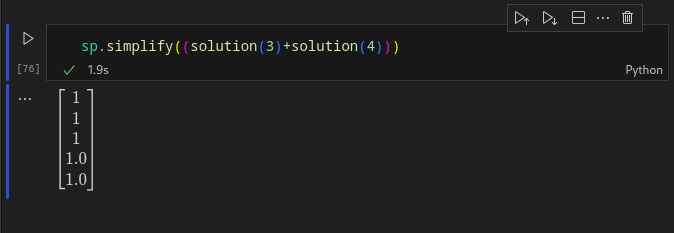
\includegraphics[width=0.8\textwidth]{../pictures/ex2-1.png}
\end{figure}

\[ g_D + g_E = 1_5\]

\subsubsection*{Caso $\boldsymbol{m = C}$:}
Then, $\gamma = 1$ and $M = \{C,D,E\}$. And so, the symbolic calculator gives us
\renewcommand*{\arraystretch}{1.7}
\[\everymath{\displaystyle} g_C = \left[\begin{matrix}\frac{\beta + \varepsilon - 1}{\beta - 1}\\\frac{\beta + \varepsilon - 1}{\beta - 1}\\1\\0\\0\end{matrix}\right], \hspace*{2em}
g_D = \left[\begin{matrix}\;0\;\\\;0\;\\\;0\;\\\;1\;\\\;0\;\end{matrix}\right], \hspace*{2em}
g_E =\left[\begin{matrix}- \frac{\varepsilon}{\beta - 1}\\- \frac{\varepsilon}{\beta - 1}\\0\\0\\1\end{matrix}\right] \]

\subsubsection*{Caso $\boldsymbol{m = B}$:}
\begin{itemize}
    \item $M = \{B,D,E\}$
    \[ \everymath{\displaystyle} g_B = \left[\begin{matrix}1\\1\\\frac{\delta + \gamma - 1}{\gamma - 1}\\0\\0\end{matrix}\right], \hspace*{2em}
    g_D = \left[\begin{matrix}0\\0\\- \frac{\delta}{\gamma - 1}\\1\\0\end{matrix}\right], \hspace*{2em}
    g_E = \left[\begin{matrix}\;0\;\\\;0\;\\\;0\;\\\;0\;\\\;1\;\end{matrix}\right] \]
    \item $M = \{B,C,D,E\}$
    \renewcommand*{\arraystretch}{1}
    \[  
    g_B = \left[\begin{matrix}1\\1\\0\\0\\0\end{matrix}\right], \hspace*{2em}
    g_C = \left[\begin{matrix}0\\0\\1\\0\\0\end{matrix}\right], \hspace*{2em}
    g_D = \left[\begin{matrix}0\\0\\0\\1\\0\end{matrix}\right], \hspace*{2em}
    g_E = \left[\begin{matrix}0\\0\\0\\0\\1\end{matrix}\right]\]
\end{itemize}

\subsubsection*{Caso $\boldsymbol{m = A}$:}
\begin{itemize}
    \item $M = \{A,D,E\}$
    \[\hspace*{-4em}\renewcommand*{\arraystretch}{1.7}\everymath{\displaystyle} g_A = \left[\begin{matrix}1\\\frac{\beta \delta + \beta \gamma - \beta + \delta \varepsilon - \delta + \gamma \varepsilon - \gamma - \varepsilon + 1}{\beta \gamma - \beta - \gamma + 1}\\\frac{\delta + \gamma - 1}{\gamma - 1}\\0\\0\end{matrix}\right], \hspace*{2em}
    g_D = \left[\begin{matrix}0\\\frac{\delta \left(- \beta - \varepsilon + 1\right)}{\beta \gamma - \beta - \gamma + 1}\\- \frac{\delta}{\gamma - 1}\\1\\0\end{matrix}\right], \hspace*{2em}
    g_E = \left[\begin{matrix}0\\- \frac{\varepsilon}{\beta - 1}\\0\\0\\1\end{matrix}\right] \]

    \item $M = \{A,C,D,E\}$
    \[\hspace*{-4em}\renewcommand*{\arraystretch}{1}\everymath{\displaystyle}
    g_A = \left[\begin{matrix}1\\0\\0\\0\\0\end{matrix}\right], \hspace*{2em}
    g_B =\left[\begin{matrix}0\\\frac{\beta + \varepsilon - 1}{\beta - 1}\\1\\0\\0\end{matrix}\right], \hspace*{2em}
    g_D = \left[\begin{matrix}0\\0\\0\\1\\0\end{matrix}\right], \hspace*{2em}
    g_E = \left[\begin{matrix}0\\- \frac{\varepsilon}{\beta - 1}\\0\\0\\1\end{matrix}\right]
      \]

    \item $M = \{A,B,D,E\}$
    \[\hspace*{-4em}\renewcommand*{\arraystretch}{1}\everymath{\displaystyle}
    g_A = \left[\begin{matrix}1\\0\\\frac{\delta + \gamma - 1}{\gamma - 1}\\0\\0\end{matrix}\right], \hspace*{2em}
    g_B = \left[\begin{matrix}0\\1\\0\\0\\0\end{matrix}\right], \hspace*{2em}
    g_D = \left[\begin{matrix}0\\0\\- \frac{\delta}{\gamma - 1}\\1\\0\end{matrix}\right], \hspace*{2em}
    g_E = \left[\begin{matrix}0\\0\\0\\0\\1\end{matrix}\right] \]

    \item $M = \{A,B,C,D,E\}$
    \[ \hspace*{-4em}\renewcommand*{\arraystretch}{1}\everymath{\displaystyle}
    g_A = \left[\begin{matrix}1\\0\\0\\0\\0\end{matrix}\right], \hspace*{2em}
    g_B = \left[\begin{matrix}0\\1\\0\\0\\0\end{matrix}\right], \hspace*{2em}
    g_C = \left[\begin{matrix}0\\0\\1\\0\\0\end{matrix}\right], \hspace*{2em}
    g_D = \left[\begin{matrix}0\\0\\0\\1\\0\end{matrix}\right], \hspace*{2em}
    g_E = \left[\begin{matrix}0\\0\\0\\0\\1\end{matrix}\right] \]
\end{itemize}

In all of the cases, the sum of vectors gives $1$ on every entry.

\subsection*{Part (e)}

$\delta$ dictates how probable is to end the random walk going from $C$ to $D$ while $\varepsilon$ dictates how probable is to end the random walk going from $B$ to $E$. Therefore, $g_D$ increases and $g_E$ decreases when we increase $\delta$, while the oposite happens when we increase $\varepsilon$.